\documentclass[reprint,english,notitlepage]{revtex4-2}
\usepackage{amsmath}
\usepackage[mathletters]{ucs}
\usepackage[utf8x]{inputenc}
\usepackage[english]{babel}
\usepackage{esint}
\usepackage{physics,amssymb}
\usepackage{graphicx}
\usepackage{xcolor}
\usepackage{hyperref}
\usepackage{listings}
\usepackage{subfigure}
% \usepackage[style=science, backend=biber]{biblatex}
% \addbibresource{References_Part_4.bib} TODO: Slett før innlevering
\hypersetup{
    colorlinks,
    linkcolor={red!50!black},
    citecolor={blue!50!black},
    urlcolor={blue!80!black}}

\lstset{inputpath=,
	backgroundcolor=\color{white!88!black},
	basicstyle={\ttfamily\scriptsize},
	commentstyle=\color{magenta},
	language=Python,
	morekeywords={True,False},
	tabsize=4,
	stringstyle=\color{green!55!black},
	frame=single,
	keywordstyle=\color{blue},
	showstringspaces=false,
	columns=fullflexible,
	keepspaces=true}


\begin{document}



\title{Onboard Orientation Software}
\author{Oskar Idland \& Jannik Eschler}
\date{\today}
\affiliation{Institute of Theoretical Astrophysics, University of Oslo}

\begin{abstract}
    This is an abstract \colorbox{red}{Complete this summary at the end of the paper}
\end{abstract}
\maketitle

\section{Introduction} \label{sec:introduction}
As there is no up or down in space we will have to create our own way of navigating the cosmos.
For this purpose, software capable of orientation in space needs to be created.
Without it, we wouldn't be able to steer our spacecraft and reach our destination.
To orient ourselves, three things will be required.\\
To know where our spacecraft is located in the solar system, we need to know our position.
The position can be found using a process called trilateration.\\
Trilateration is the process by which one determines the position of a body using measured distances to known positions.%~\parencite[][]{Relevant_theory}\\ 
TODO: % Ta bort kommentar 
This means we can use measure distances from the spacecraft to object for which we know the position and calculate our own position from there.
These measurements will be done by our onboard radar array.\\
The software for the array includes an index of all known objects in our solar system and can therefore include the radius of the object in it's calculations.
The measured distance will therefore always be from the spacecraft to the center of the object.\\
As most objects in space - including the spacecraft itself - are moving, we need to specify the point in time when the measurements were taken.
Otherwise, we could not know the exact location of the object we are measuring the distance to.\\
Furthermore, we need to know in which direction we are moving.
This consists of two parts. First, we create a reference picture of the universe in all directions with the earth in the center. Second, we take a picture on our shuttle and compare that picture with the reference picture to calculate which direction we are looking.\\
We also need to know the velocity of the spacecraft relative to the star in our solar system.
To find the velocity relative to a star, we can use a phenomenon called Doppler shift.
Electromagnetic radiation consist of waves which have an amplitude and a frequency.
The amplitude determines the intensity of the light, whereas the frequency determines the energy of the wave, or in other words the colour.
If two objects move at high velocities relative to each other and one receives light sent out by the other, the electromagnetic wave appears to be compressed if the objects are moving towards each other and stretched out if they are moving away from each other.
Therefore, the frequency will appear to be higher or lower respectively.
Additionally, relativistic effects distort the wave further due to the relatively high speeds.\\
However, we cannot apply this directly to find our velocity relative to the star in our solar system as this only determines the radial velocity relative to the star and the spacecraft also has a tangential velocity to relative to the star.
We will therefore use reference stars which are outside our solar system.\\
The Doppler shift and therefore the velocity of the reference relative to the star in our solar system is known.
We can then measure the Doppler shift of the reference stars from our spacecraft and determine the velocity of the stars relative to the spacecraft.
Here, we assume the lines from the spacecraft to the reference stars and the lines from the star in our solar system to the reference stars to be parallel due to the reference stars being very far away.\\
These velocities can then be used to find the velocity of the spacecraft relative to the star in our solar system.
Since we are only able to find the radial velocity to the reference star, we will need at least two stars to be able to determine our velocity in two dimensions.\\
As stars mainly consist of hydrogen, most electromagnetic radiation sent out from stars will be from hydrogen atoms sending out radiation.
This spike in the amount of radiation at a specific wavelength is called the $H_{\alpha}$ Spectral Line, which has a wavelength of 656.3 nanometers.\\
To be able to do all calculations, a cartesian coordinate system will be used with the star in our solar system being in the origin and the x-axis pointing at the position of planet 0 at $T = 0$.

\section{Theory} \label{sec:theory}
% For theory, see section Relevant Mathematics in the project description~\parencite[][]{Relevant_theory}

\section{Method} \label{sec:method}
\subsection{Generating Pictures} \label{subsec: generating pictures}


A satellite is orbiting our home planet and has taken a $ 180 ^{o} \times 360 ^{o} $ picture of the entire sky where all positions are described using spherical coordinates. As the stars and galaxies as very far away we are going to assume the pictures looks the same from the perspective of our shuttle. Using this picture we can create a stereographic projection as a means to convert from spherical coordinates to planar coordinates. Comparing the picture taken from a camera at on the shuttle we can find our orientation.
\begin{figure}[h!]
  \centering
  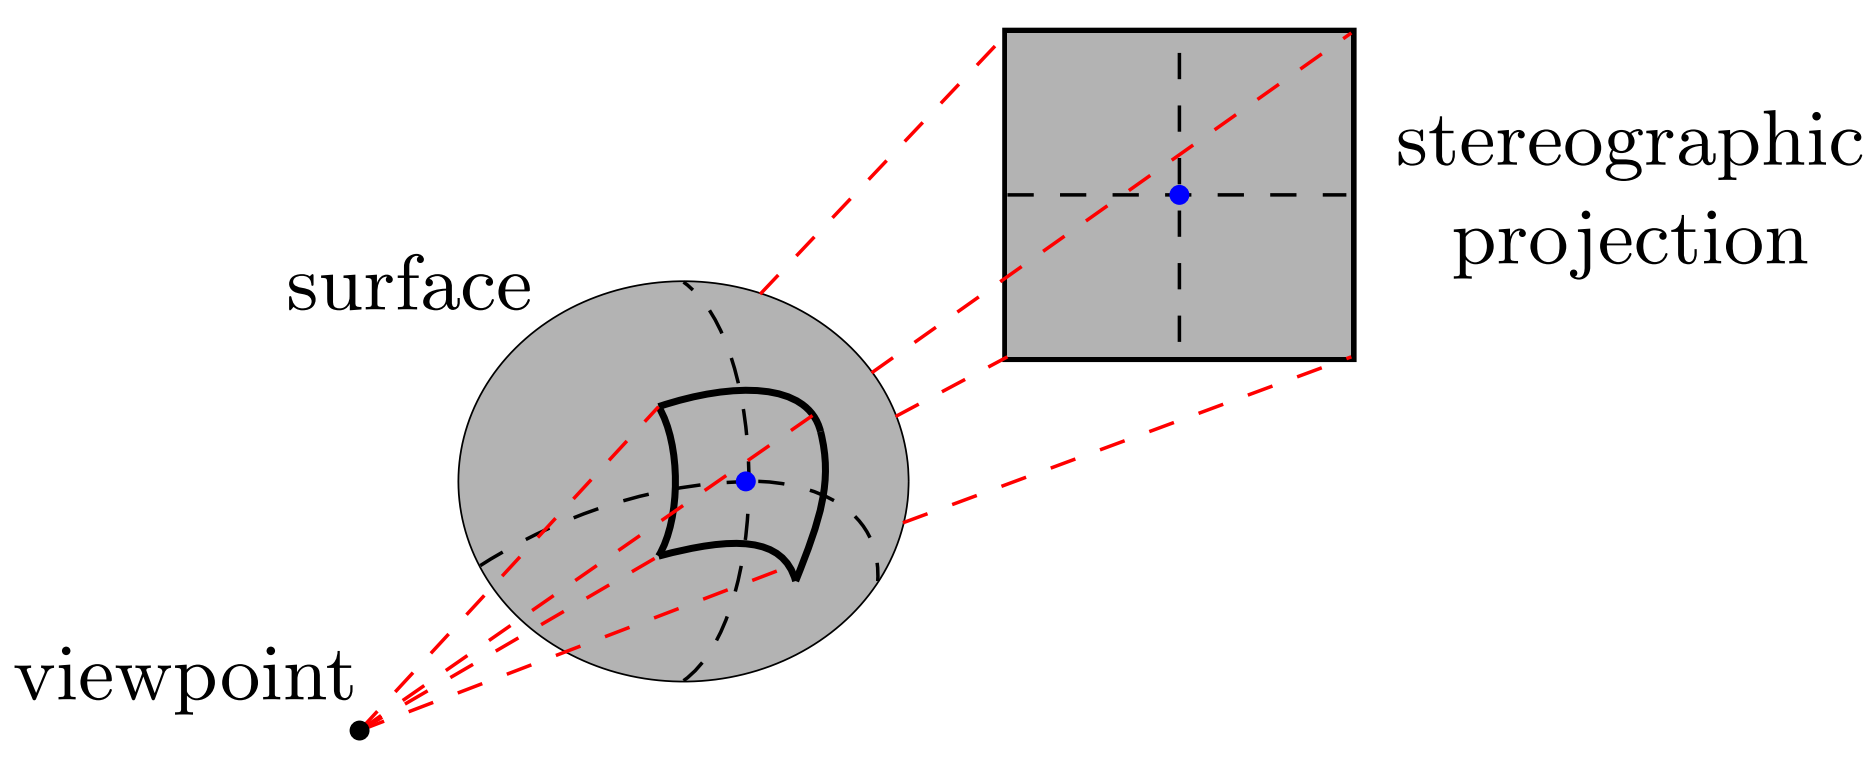
\includegraphics[scale = .2]{Figures/Stereographic_projection}
  \caption{Illustration of stereographic projection}
  \label{fig: Stereographic Projection}
\end{figure}\\

To relate the spherical coordinates $ (\theta, \phi) $ to the planar coordinates $ (X, Y) $ we use the following equations:
\begin{subequations}
	\begin{equation} \label{Spherical to X}
		X = κ  \sin θ \sin (ϕ - ϕ _0)
	\end{equation}
	\begin{equation}\label{Spherical to Y}
		Y = κ (\sin θ _0 \cos  θ - \cos θ _0 \sin θ \cos (ϕ - ϕ _0))  
	\end{equation}
	
	\begin{equation} \label{eq: kappa}
	  \kappa = \frac{2}{1 + \cos \theta _{0}\cos \theta + \sin \theta _{0} \sin \theta \cos (\phi - \phi _{0})}
	\end{equation}
\end{subequations}

To relate planar coordinates $ X,Y $ with spherical coordinates $ ϕ, θ $ we use the following equations 

\begin{subequations} \label{eq: planar to spherical coordinates}
	\begin{equation}
	  \theta = \theta_0 - \arcsin \left[ \cos β \cos θ _{0} + \frac{Y}{\rho} \sin β \sin θ _{0}\right] 
	\end{equation}
	\begin{equation}
	  \phi = \phi _{0} + \arctan \left[ \frac{X \sin \beta}{\rho \sin \theta _{0} \cos \beta - Y \cos  \theta _{0} \sin  \beta} \right] 
	\end{equation}
  \end{subequations}


Using equations \ref{eq: planar to spherical coordinates} we can convert the data taken from the satellite containing values for $ X,Y  $ and the color of the pixel in the RGB format, into a reverse stereographic projection in the $ ϕ, \theta $ -plane. This gives us a complete reference picture using spherical coordinates!

When the camera onboard takes a pictures it will be limited by its field of view (FOV). The FOV will be described as the maximum angular width $ \alpha $ of the photo. We use the following equations to define it. 
\begin{equation} \label{eq: max angular width}
	α _{\theta} = θ _{max} - \theta _{min}, \quad α _{\phi} = ϕ _{max} - ϕ _{min}
\end{equation}

This creates ranges of coordinates for $\theta$ and $\phi$:
\begin{equation}\label{eq: limitations phi and theta}
  - \frac{\alpha _{\theta}}{2} \le θ - θ _{0} \le \frac{\alpha _{\theta }}{2}, \quad - \frac{\alpha _{\theta}}{2} \le ϕ  - ϕ _{0} \le \frac{\alpha _{\theta }}{2}
\end{equation}

This, in turn, also creates limitations on the coordinates $ (X,Y) $ of the stereographic projection derrived in \ref{ssec: lim x,y}: 
\begin{subequations} \label{eq: limitations X and Y lim}
	\begin{equation}
		X _{max / min} = ± \frac{2 \sin (α _{\phi} / 2)}{1 + \cos (\alpha _{\phi})}
	  \end{equation}
	  
	  
	\begin{equation}
		Y _{max / min} ± \frac{2 \sin (\alpha _{\theta}  / 2)}{1 + \cos (α _{\theta}/2)}
	\end{equation}
	
\end{subequations}
This is the key to generating a grid of x and y values which we will base our position from later. 

To help us check that our calculations are correct we have been given a sample picture we will recreate using equations \ref{eq: planar to spherical coordinates}
The picture is centered around $ \phi = 0^{o} $ and $ \theta = 90^{o} $. The camera used has a FOV of $ \alpha_{\theta} = \alpha_{\phi} = 70^{o} $. To get the full range of the coordinates $ (X,Y) $ we simply find the height and width of the array containing the data. With this information we are able to recreate the same picture~\ref{fig: ref picture}


\subsection{Image Analysis} \label{ssec: image analysis}
We have assumed that $ \theta_{0} = \frac{\pi}{2} $ for the entire trip which means there is only one variable, the angle which the picture is centered around $ \phi_{new} $. A simple solution can be implemented assuming the space shuttle only turns at integer angle values. First, we create an Image object using the PIL module. Then we iterate over all angles $ \phi \in  \left\{ 0^{o}, 1^{o}, 2^{o} \dots 359 ^{o} \right\}  $ and compare the Image with the ones we created ourselves. Once we get a match we know our $ \phi _{0} $.



\subsection{Determining the velocity}\label{subsec:determining-the-velocity}
As explained in section~\ref{sec:introduction}, the velocity relative to the star will be determining using an effect called the Doppler shift.
When tasked to do so, the onboard equipment of the spacecraft can now determine the Doppler shift $\Delta \lambda$ of the $H_{\alpha}$ Spectral line.\\
It must be noted that all these measurements will be done at the time $T_M$.\\
The angles from the x-axis at which the reference stars $Star_{R1}$ and $Star_{R2}$ lie are known as $\phi_1 = 281.057^{\circ}$ and $\phi_2 = 157.433^{\circ}$.
These have been obtained beforehand by our astronomers.
Now the velocities $v_{phi1}$ and $v_{phi2}$ in the direction of these angles can be determined by measuring the Doppler shift $\Delta \lambda$ and using the relationship between the Doppler shift and the velocity~\eqref{Dopplershift1}
\begin{align}
    \frac{\Delta \lambda}{\lambda_0} &= \frac{v_{rad}}{c} \label{Dopplershift1}\\
	v_{rad} &= \frac{\Delta \lambda}{\lambda_0} c \label{Dopplershift2}
\end{align}
With $\lambda_0$ being the wavelength of the observed electromagnetic wave from an observer at rest, $c$ being the speed of light and $v_{rad}$ being the velocity of the two objects relative to each other.\\
Given the velocity in the direction of the two stars, we will need to change our coordinate system to calculate the velocity of the spacecraft.
The new unit vectors of our coordinate system will be given by
\begin{align}\label{Coord_chg1}
\begin{pmatrix}
    \hat{u}_1 \\
	\hat{u}_2
\end{pmatrix} =
\begin{pmatrix}
    \cos \phi_1 & \sin \phi_1\\
	\cos \phi_2 & \sin \phi_2
\end{pmatrix}
\end{align}
Now, we are able to determine to calculate the velocity of the spacecraft, and the velocity of the star in our solar system relative to the two reference stars in our new coordinate system.\\
To find the velocity of the spacecraft relative to the star in our solar system, we can simply subtract the velocity of the star in our system from the velocity of the spacecraft.
\[
v_u = v_{SC}-v_{Star}
\]
However, our orientation system works in cartesian coordinates, so will have to change our coordinate system back to the initial coordinate system.
To change back to the initial system, we invert the operations used in~\eqref{Coord_chg1} and use them on the velocity vector
$v_u = \begin{pmatrix}
    v_{u1}\\ v_{u2}
\end{pmatrix}$.

\[
    \begin{pmatrix}
        v_x\\
		v_y
    \end{pmatrix}
	 = \frac{1}{\sin\left(\phi_1 - \phi_2 \right)}
	\begin{pmatrix}
	    \sin \phi_2 & -\sin \phi_1\\
		-\cos \phi_2 & \cos \phi_1
	\end{pmatrix}
	\begin{pmatrix}
		v_{u1}\\ v_{u2}
	\end{pmatrix}
\]


\subsection{The position of the Spacecraft}\label{subsec:the-position-of-the-spacecraft}
The position of the spacecraft will be determined using the trilateration process.
This process is much used for locating purposes, which includes the global positioning system (GPS).\\
Using the onboard radar array we will be able to determine distances to the star in our solar system and other planets at a specific point in time $T_m$.
The position of the other objects has already been found as a function of time and can therefore be determined for the time $T_m$.\\
\begin{align*}
    S\left(T \right) &= \left(x_S, y_S \right)\\
	P_1\left(T \right) &= \left(x_{P1}, y_{P1} \right)\\
	P_2\left(T \right) &= \left(x_{P2}, y_{P2} \right)
\end{align*}
The radar will be used to find the distance to two planets as well as the distance to the star in our solar system.
The distance to the star in our solar system $r_S$ and the distance to the two planets $r_{P1}$ and $r_{P2}$ can be described using Pythagoras theorem.
\begin{align}
    r_S^2 &= (x_{SC} - x_S)^2 + (y_{SC} - y_S)^2 \label{r_s}\\
	r_{P1}^2 &= (x_{SC} - x_{P1})^2 + (y_{SC} - y_{P1})^2 \label{r_p1}\\
	r_{P2}^2 &= (x_{SC} - x_{P2})^2 + (y_{SC} - y_{P2})^2  \label{r_p2}
\end{align}
The setup for the calculations has been visualised in figure~\ref{fig:trilateration_figure} .
\begin{figure}[h]
	%% H(Here), h(here approx), t(top of page), b(bottom of page)
	\centering
	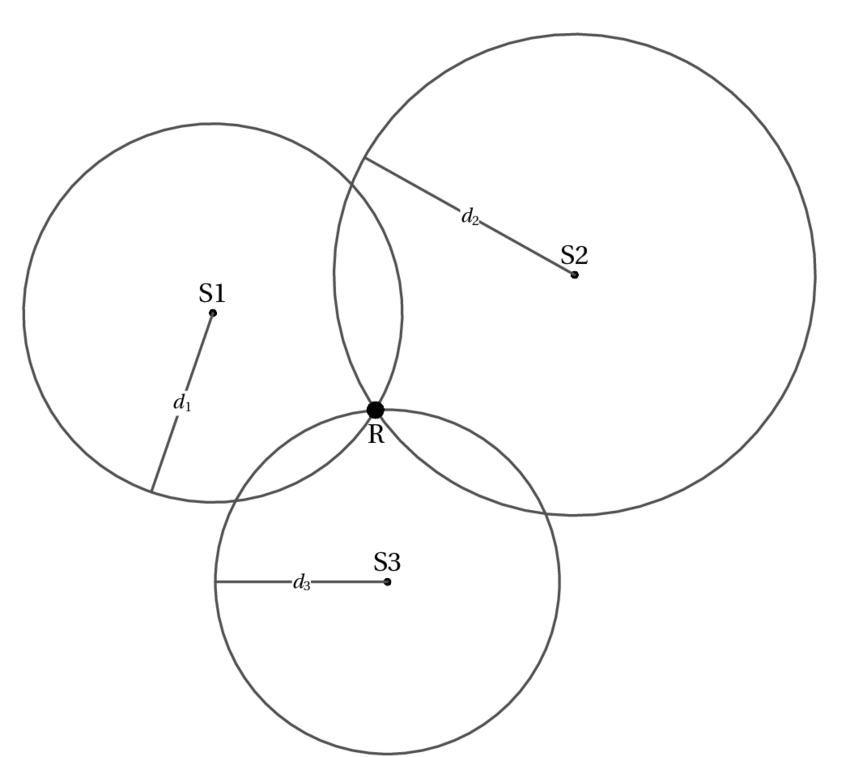
\includegraphics[scale=0.2]{Figures/trilateration}
	% \caption{Visualisation of the trilateration method. From~\parencite[][]{trilateration_picture}}
	\label{fig:trilateration_figure} % TODO: Slett før innlevering
\end{figure}
Since the star will always be in the origin of the coordinate system, $r_S$ can be simplified to
\begin{align*}
    r_S^2 &= x_{SC}^2 + y_{SC}^2
\end{align*}
Solving the equation set consisting of equations~\eqref{r_s},~\eqref{r_p1} and~\eqref{r_p2} for $x_{SC}$ and $y_{SC}$ yields
\begin{align*}
    A& = \left(-2x_S + 2x_{P1}\right)\\
	B& = \left(-2y_S + 2y_{P1}\right)\\
	C& = r_S^2 - r_{P1}^2 - x_S^2 + x_{P1}^2 - y_S^2 + y_{P1}^2\\
	D& = \left(-2x_{P1} + 2x_{P2}\right)\\
	E& = \left(-2y_{P1} + 2y_{P2}\right)\\
	F& = r_{P1}^2 - r_{P2}^2 - x_{P1}^2 + x_{P2}^2 - y_{P1}^2 + y_{P2}^2
\end{align*}
\begin{align*}
    x_{SC}& = \frac{CE - FB}{EA - BD}\\
	y_{SC}& = \frac{CD - AF}{BD - AE}
\end{align*}
% The calculations for this are based on the calculations from~\parencite[][]{trilateration} TODO: Slett før innlevering
The position of the spacecraft $SC$ is then given by
\begin{align*}
    SC = \left(x_{SC}, y_{SC} \right)
\end{align*}



\section{Results} \label{sec:results}
We have now tested the orientation software for our rocket right after our rocket has reached space, or in other words, reached exit velocity.
First, we have used our onboard camera to take a picture in the direction, in which the spacecraft is pointing.
The picture we have received from the camera can be seen in figure~\ref{fig:sky_picture}.
This picture has then been matched with the reference picture~\ref{fig: ref picture}, which our team has made beforehand.

\begin{figure}[h]
	%% H(Here), h(here approx), t(top of page), b(bottom of page)
	\centering
	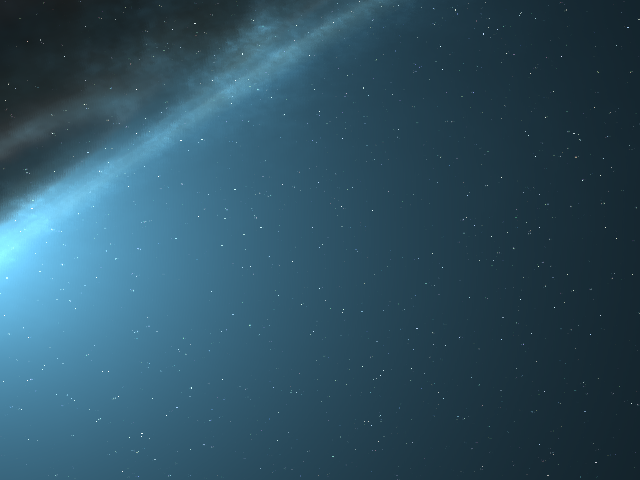
\includegraphics[scale=0.15]{Python/sky_picture}
	\caption{The image taken by the onboard camera right after the spacecraft reaches space.}\label{fig:sky_picture}
\end{figure}

\begin{figure}[h!]
	\centering
	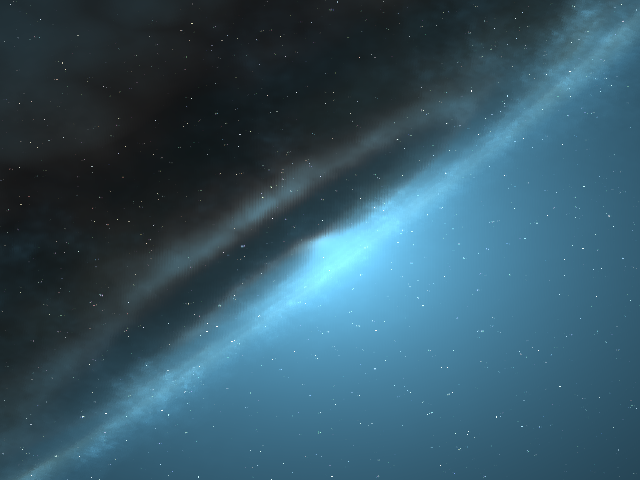
\includegraphics[scale = 0.2]{Test_Image}
	\caption{Recreated reference picture for our software %from~\parencite[][]{Relevant_theory}} TODO: Slett før innlevering%
	}
	\label{fig: ref picture}
  \end{figure}

By comparing the picture taken right after reaching space to different parts of the reference picture, we found the angle of the spacecraft right after reaching space to be $39^{\circ}$.\\

At the same time, the distances from the spacecraft to the star in our solar system, planet 3 and planet 6 have been measured.
The distances from the spacecraft to the different bodies are
\begin{align*}
    r_{Star} = 9.31411 \,AU\\
	r_{P3} = 56.16394 \,AU\\
	r_{P6} = 47.86636 \,AU\\
\end{align*}
These distances have then been used to triangulate the position of the spacecraft right after reaching outer space using the method described in section~\ref{subsec:the-position-of-the-spacecraft}.
This amounted to the position of the spacecraft being $SC = (9.3141, 1.2278 \times 10^{-4}) AU$.\\

Furthermore, the velocity of the spacecraft of the spacecraft has been calculated using the methods from section~\ref{subsec:determining-the-velocity}.
The dopplershifts $\Delta\lambda_{SC1}$ and $\Delta\lambda_{SC2}$ of the $H_{\alpha}$ spectral line from the two reference stars at the angles $ \phi_1 = 281.057^{\circ}$ and $ \phi_2 = 157.433^{\circ}$ have been measured using onboard instruments.
The measurements resulted in the dopplershifts at the spacecraft being
\begin{align*}
	&\Delta\lambda_{SC1} = 0.057026 \,\text{nm}\\
	&\Delta\lambda_{SC2} = 0.0048287 \,\text{nm}
\end{align*}
The dopplershifts at the star in our solar system have been predetermined by our scientist and are
\begin{align*}
    &\Delta\lambda_{ST1} = 0.017867 \,\text{nm}\\
	&\Delta\lambda_{ST2} = -0.0042600 \,\text{nm}
\end{align*}
Using these measurements, the velocity $v_{SC}$ of the spacecraft has been determined to be
\begin{align*}
    v_{SC} = (2.7712, 4.3863) \,\text{AU/Year}
\end{align*}

By combining all these measurements and results, we were successfully able to determine the position fo the spacecraft when reaching space after launching.\\
After successfully determining the position after reaching space, the software has been uploaded to the spacecrafts main computer.
This means, the spacecraft will be able to do all the calculations, and therefore orient itself by sending a simple command to it.

\section{Discussion} \label{sec:discussion}
The software is able to accurately recreate the sample picture we were given.
It is also able to accurately tell which direction the shuttle is pointing, with the caveat being the angle must be an integer value.
This is caused by the local database onboard is based of the full picture taken by the satellite orbiting our planet.
We defined each picture to have a distance of 1 degree which limits the use cases.

This could become a problem.
Luckily our shuttle is able to take millions of picture per second so we have a wide range to work with.
The super computer onboard will easily go through all pictures and find a match in no time.
This makes the odds of failure to find a picture insignificant.


\section{Conclusion} \label{sec:conclusion}



\section{Appendix: Mathematical Derivations}
\subsection{Calculating the limitations on $ X $ and $ Y $.} \label{ssec: lim x,y}

\[
	X = \kappa  \sin \theta \sin (ϕ - ϕ _0)
\]
To make it easier to find the limitations we set $ X = 0 $. 
\[
\kappa \sin \theta \sin (ϕ - ϕ _0) = 0
\]
Inserting the definition of $ \kappa $ from equation \ref{eq: kappa}:
\[
	\frac{2 \sin θ \sin (ϕ - ϕ _0)}{1 + \cos \theta _{0}\cos \theta + \sin \theta _{0} \sin \theta \cos (\phi - \phi _{0})} = 0
\]
Inserting the ranges of values for $ \theta $ and $ \theta_0 $ from equation~\ref{eq: limitations phi and theta}, we get the upper and lower limit of what equations to solve.
\[
\frac{2 \sin  θ \sin (\pm α_ϕ / 2)}{1 + \cos θ_0 \cos θ + \sin θ_0 \sin  θ \cos (\pm α_ϕ / 2)} = 0
\]


\newpage
%\printbibliography 
TODO: % Ta bort kommentar

\end{document}